%%%%%%%%%%%%%%%%%%%%%%%%%%%%%%%%%%%%%%%%%
% Beamer Presentation
% LaTeX Template
% Version 1.0 (10/11/12)
%
% This template has been downloaded from:
% http://www.LaTeXTemplates.com
%
% License:
% CC BY-NC-SA 3.0 (http://creativecommons.org/licenses/by-nc-sa/3.0/)
%
%%%%%%%%%%%%%%%%%%%%%%%%%%%%%%%%%%%%%%%%%

%----------------------------------------------------------------------------------------
%	PACKAGES AND THEMEShttps://www.overleaf.com/project/5dbfadb88b2560000102ab44
%----------------------------------------------------------------------------------------

\documentclass{beamer}

\mode<presentation> {

% The Beamer class comes with a number of default slide themes
% which change the colors and layouts of slides. Below this is a list
% of all the themes, uncomment each in turn to see what they look like.

%\usetheme{default}
%\usetheme{AnnArbor}
%\usetheme{Antibes}
%\usetheme{Bergen}
%\usetheme{Berkeley}
%\usetheme{Berlin}
\usetheme{Boadilla}
%\usetheme{CambridgeUS}
%\usetheme{Copenhagen}
%\usetheme{Darmstadt}
%\usetheme{Dresden}
%\usetheme{Frankfurt}
%\usetheme{Goettingen}
%\usetheme{Hannover}
%\usetheme{Ilmenau}
%\usetheme{JuanLesPins}
%\usetheme{Luebeck}
%\usetheme{Madrid}
%\usetheme{Malmoe}
%\usetheme{Marburg}
%\usetheme{Montpellier}
%\usetheme{PaloAlto}
%\usetheme{Pittsburgh}
%\usetheme{Rochester}
%\usetheme{Singapore}
%\usetheme{Szeged}
%\usetheme{Warsaw}

% As well as themes, the Beamer class has a number of color themes
% for any slide theme. Uncomment each of these in turn to see how it
% changes the colors of your current slide theme.

%\usecolortheme{albatross}
%\usecolortheme{beaver}
%\usecolortheme{beetle}
%\usecolortheme{crane}
%\usecolortheme{dolphin}
%\usecolortheme{dove}
%\usecolortheme{fly}
%\usecolortheme{lily}
%\usecolortheme{orchid}
%\usecolortheme{rose}
%\usecolortheme{seagull}
%\usecolortheme{seahorse}
%\usecolortheme{whale}
\usecolortheme{wolverine}

%\setbeamertemplate{footline} % To remove the footer line in all slides uncomment this line
\setbeamertemplate{footline}[page number] % To replace the footer line in all slides with a simple slide count uncomment this line

\setbeamertemplate{navigation symbols}{} % To remove the navigation symbols from the bottom of all slides uncomment this line
}

\setbeamertemplate{bibliography item}{\insertbiblabel}


\usepackage{graphicx} % Allows including images
\usepackage{booktabs} % Allows the use of \toprule, \midrule and \bottomrule in tables
%\usepackage {tikz}
\usepackage{tkz-graph}
\usepackage{bibentry}


\usepackage[
backend=biber,
style=numeric,
sorting=ynt
]{biblatex}
 
\documentclass[xcolor=table]{beamer} 

\bibliography{bibfile}

\graphicspath{ {images/} }

\GraphInit[vstyle = Shade]
\tikzset{
  LabelStyle/.style = { rectangle, rounded corners, draw,
                        minimum width = 2em, fill = yellow!50,
                        text = red, font = \bfseries },
  VertexStyle/.append style = { inner sep=5pt,
                                font = \normalsize\bfseries},
  EdgeStyle/.append style = {->, bend left} }
\usetikzlibrary {positioning}
%\usepackage {xcolor}
\definecolor {processblue}{cmyk}{0.96,0,0,0}

% show sections only
\setcounter{tocdepth}{1}
% show subsections
%\setcounter{tocdepth}{2}
% show subsubsections
%\setcounter{tocdepth}{3}
\AtBeginSection[]
{
    \begin{frame}
        \frametitle{Table of Contents}
        \tableofcontents[currentsection]
    \end{frame}
}

%\AtBeginSubsection[]
%{
%    \begin{frame}
%        \frametitle{Table of Contents}
%        \tableofcontents[currentsection,currentsubsection]
%    \end{frame}
%}

%----------------------------------------------------------------------------------------
%	TITLE PAGE
%----------------------------------------------------------------------------------------

\title[Short title]{caDDS: Community Assisted Distributed Database for Sequences} % The short title appears at the bottom of every slide, the full title is only on the title page


%%%%%%%%%%%%%%%%%%%%%%%%%%% INFO %%%%%%%%%%%%%%%%%%%%%%%%%%%%%%%%%%%%%%%%%%%%%%%%%

\author{Azcarraga, Araya} % Your name
\institute[Department of Computer Science, University of the Philippine - Diliman] % Your institution as it will appear on the bottom of every slide, may be shorthand to save space
{
University of the Philippine - Diliman\\ % Your institution for the title page
\medskip
}
\date{\today} % Date, can be changed to a custom date


%----------------------------------------------------------------------------------------
%	PRESENTATION SLIDES
%----------------------------------------------------------------------------------------


\begin{document}


%%%%%%%%%%%%%%%%%%%%%%%%%%%%% OVERVIEW %%%%%%%%%%%%%%%%%%%%%%%%%%%%%%%%%%%%%%%%%%%%%%
\begin{frame}
\frametitle{Overview} % Table of contents slide, comment this block out to remove it
\tableofcontents % Throughout your presentation, if you choose to use \section{} and \subsection{} commands, these will automatically be printed on this slide as an overview of your presentation
\end{frame}


%%%%% TODO
%% READ COMMENTS
%% REARRANGE SOME SLIDES
%% ADD MISSING SLIDES (KAHIT NO CONTENT) FOR NARRATIVE PURPOSES
%% REVISE SLIDES AND ADD NOTES

%%%%%%%%%%%%%%%%%%%%%%%%%%%%% INTRO + RRL %%%%%%%%%%%%%%%%%%%%%%%%%%%%%%%%%%%%%%%%%%%%%%
\section{Introduction}

    \subsection{Definition} %keep daw
    \begin{frame}{Human DNA Length}
    % mahirap maintindihan, di madali iconnect sa complexity of sequencing
    % not as connected
    % put instead another slide
    % if you unwind all the letters it reaches to the moon and back
    % represent through a sequence of letters
    % see both the complexity and the size of data
    
        \centering
        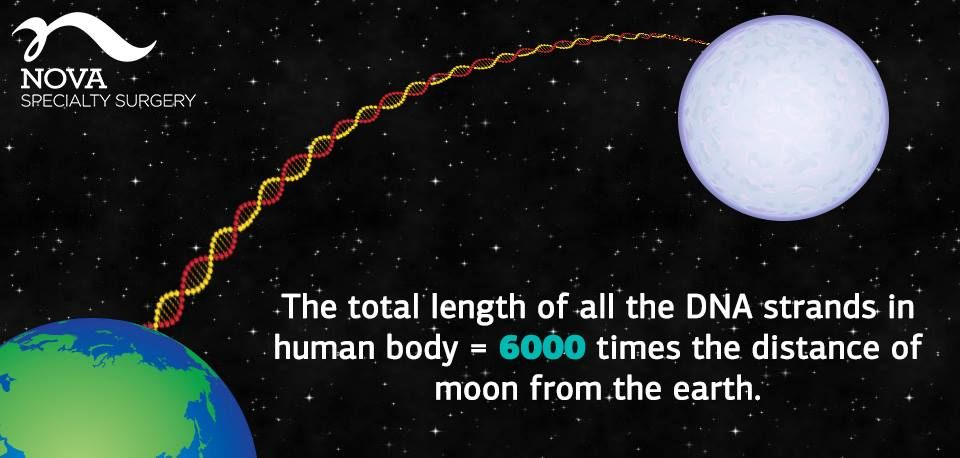
\includegraphics[scale=0.3]{dna-length.jpg}
    \end{frame}
    
    
    \begin{frame}{Definition of Genomics}
        According to the National Institute of Health \textit{Specifically for the Human Genome Project}
                \begin{block} {\textbf{Definition of Genomics}}
        Genomics is the study of all of a person's genes (the genome), including interactions of those genes with each other and with the person's environment. \cite{genomics-definition}
                \end{block}
    The genomics definition we will use is for \textbf{all} organisms
    \end{frame}
    
    
    \subsection{Introduction + RRL}
    \begin{frame}{Introduction}
    % kadugtong ng first slide
    % ATCG na paulit ulit
    % Sequence of letters codes for instructions to determine the traits of the organism
        \begin{itemize}
            \item DNA comprises of the components A,T,G,C
            \begin{itemize}
                \item \textbf{A} - Adenine
                \item \textbf{T} - Thymine
                \item \textbf{G} - Guanine
                \item \textbf{C} - Cytosine
            \end{itemize}
            \item There needs to be a lot of these components to describe complex organisms
            \begin{itemize}
                \item The full human genome contains around $3.2 x 10^9$ base pairs \cite[p.~4]{introgenomics}
            \end{itemize}
        \end{itemize}
        \centering
        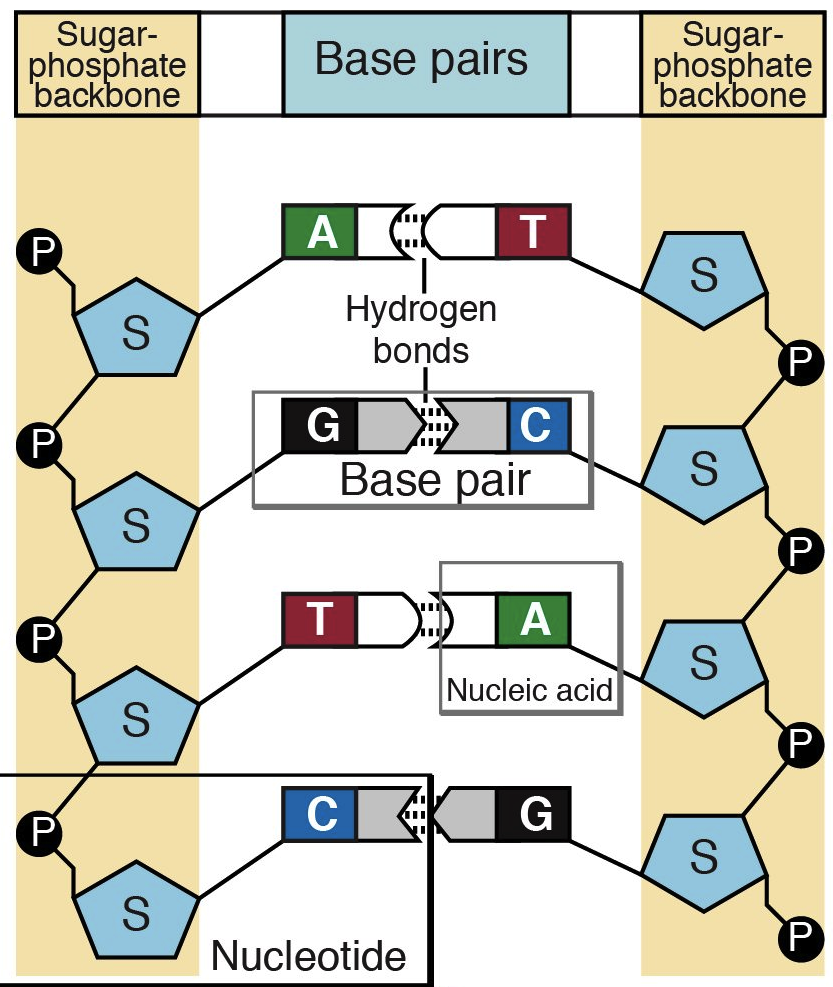
\includegraphics[scale=0.1]{gene-base-pair.png}
    \end{frame}
    
    \subsection{Genomics Data}
    \begin{frame}{Genomics Data}
    % can have billions of these...
            \textbf{Data Type}
    \begin{itemize}
        \item Store DNA sequences digitally
        \item A simple data file format is called FASTA format
            \begin{itemize}
                \item starts with $>$
                \item then can add keywords and attributes separated by $|$
            \end{itemize}
    \end{itemize}
    
    \begin{block}{Sample.FASTA}
    $>$AB000263 $|$acc=AB000263$|$descr=Homo sapiens mRNA for prepro cortistatin like peptide, complete cds.$|$len=70
ACAAGATGCCATTGTCCCCCGGCCTCCTGCTGCTGCTGCTCTCCGGGGCCACGGCCACCGCTGCCCTGCC
    \end{block}
    
    \end{frame}
    
    \subsection{Sequencing}
    \begin{frame}{Sequencing}

        \textbf{Sequencing}
    \begin{itemize}
        \item Sequencers are machines used to look at the DNA of a specimen (A,G,C,T)
        \begin{itemize}
            \item Sequencers look at the exact order of a single strand \cite{genomics-definition}. 
        \end{itemize}
        \item DNA is \textbf{replicated} and fragmented before processing
        \item Sequencers then reads (or sequences) them
        \item Output of the read fragments is contained in a .FASTA file
    \end{itemize}
            \centering
        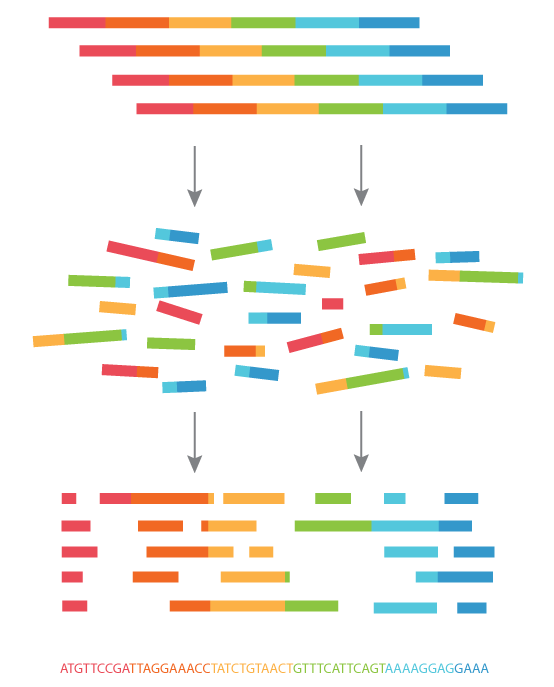
\includegraphics[scale=0.2]{sequencing.png}
    \end{frame}
    
    \begin{frame}{Next Generation Sequencing}
    (2003) The first human genome took ten years of work and $3,000,000,000$ \$ to finish.
    \begin{itemize}
        \item (2019) Currently the technology today in Japan can make 10,000 human genomes per day (Timewise: 36.5 million times faster) \cite[p.~19]{introgenomics}
    \end{itemize}
    \textbf{Next Generation Sequencers}
        \begin{itemize}
        \item Can read more faster, and cheaper
        \item More data
        \item Technology will get faster, there needs to be systems in preparation for that
    \end{itemize}
    \end{frame}
    
   \begin{frame}{Human genome cost over time}
    
    Graph of human genome cost over time \cite{genomics-cost} \\
    \centering
    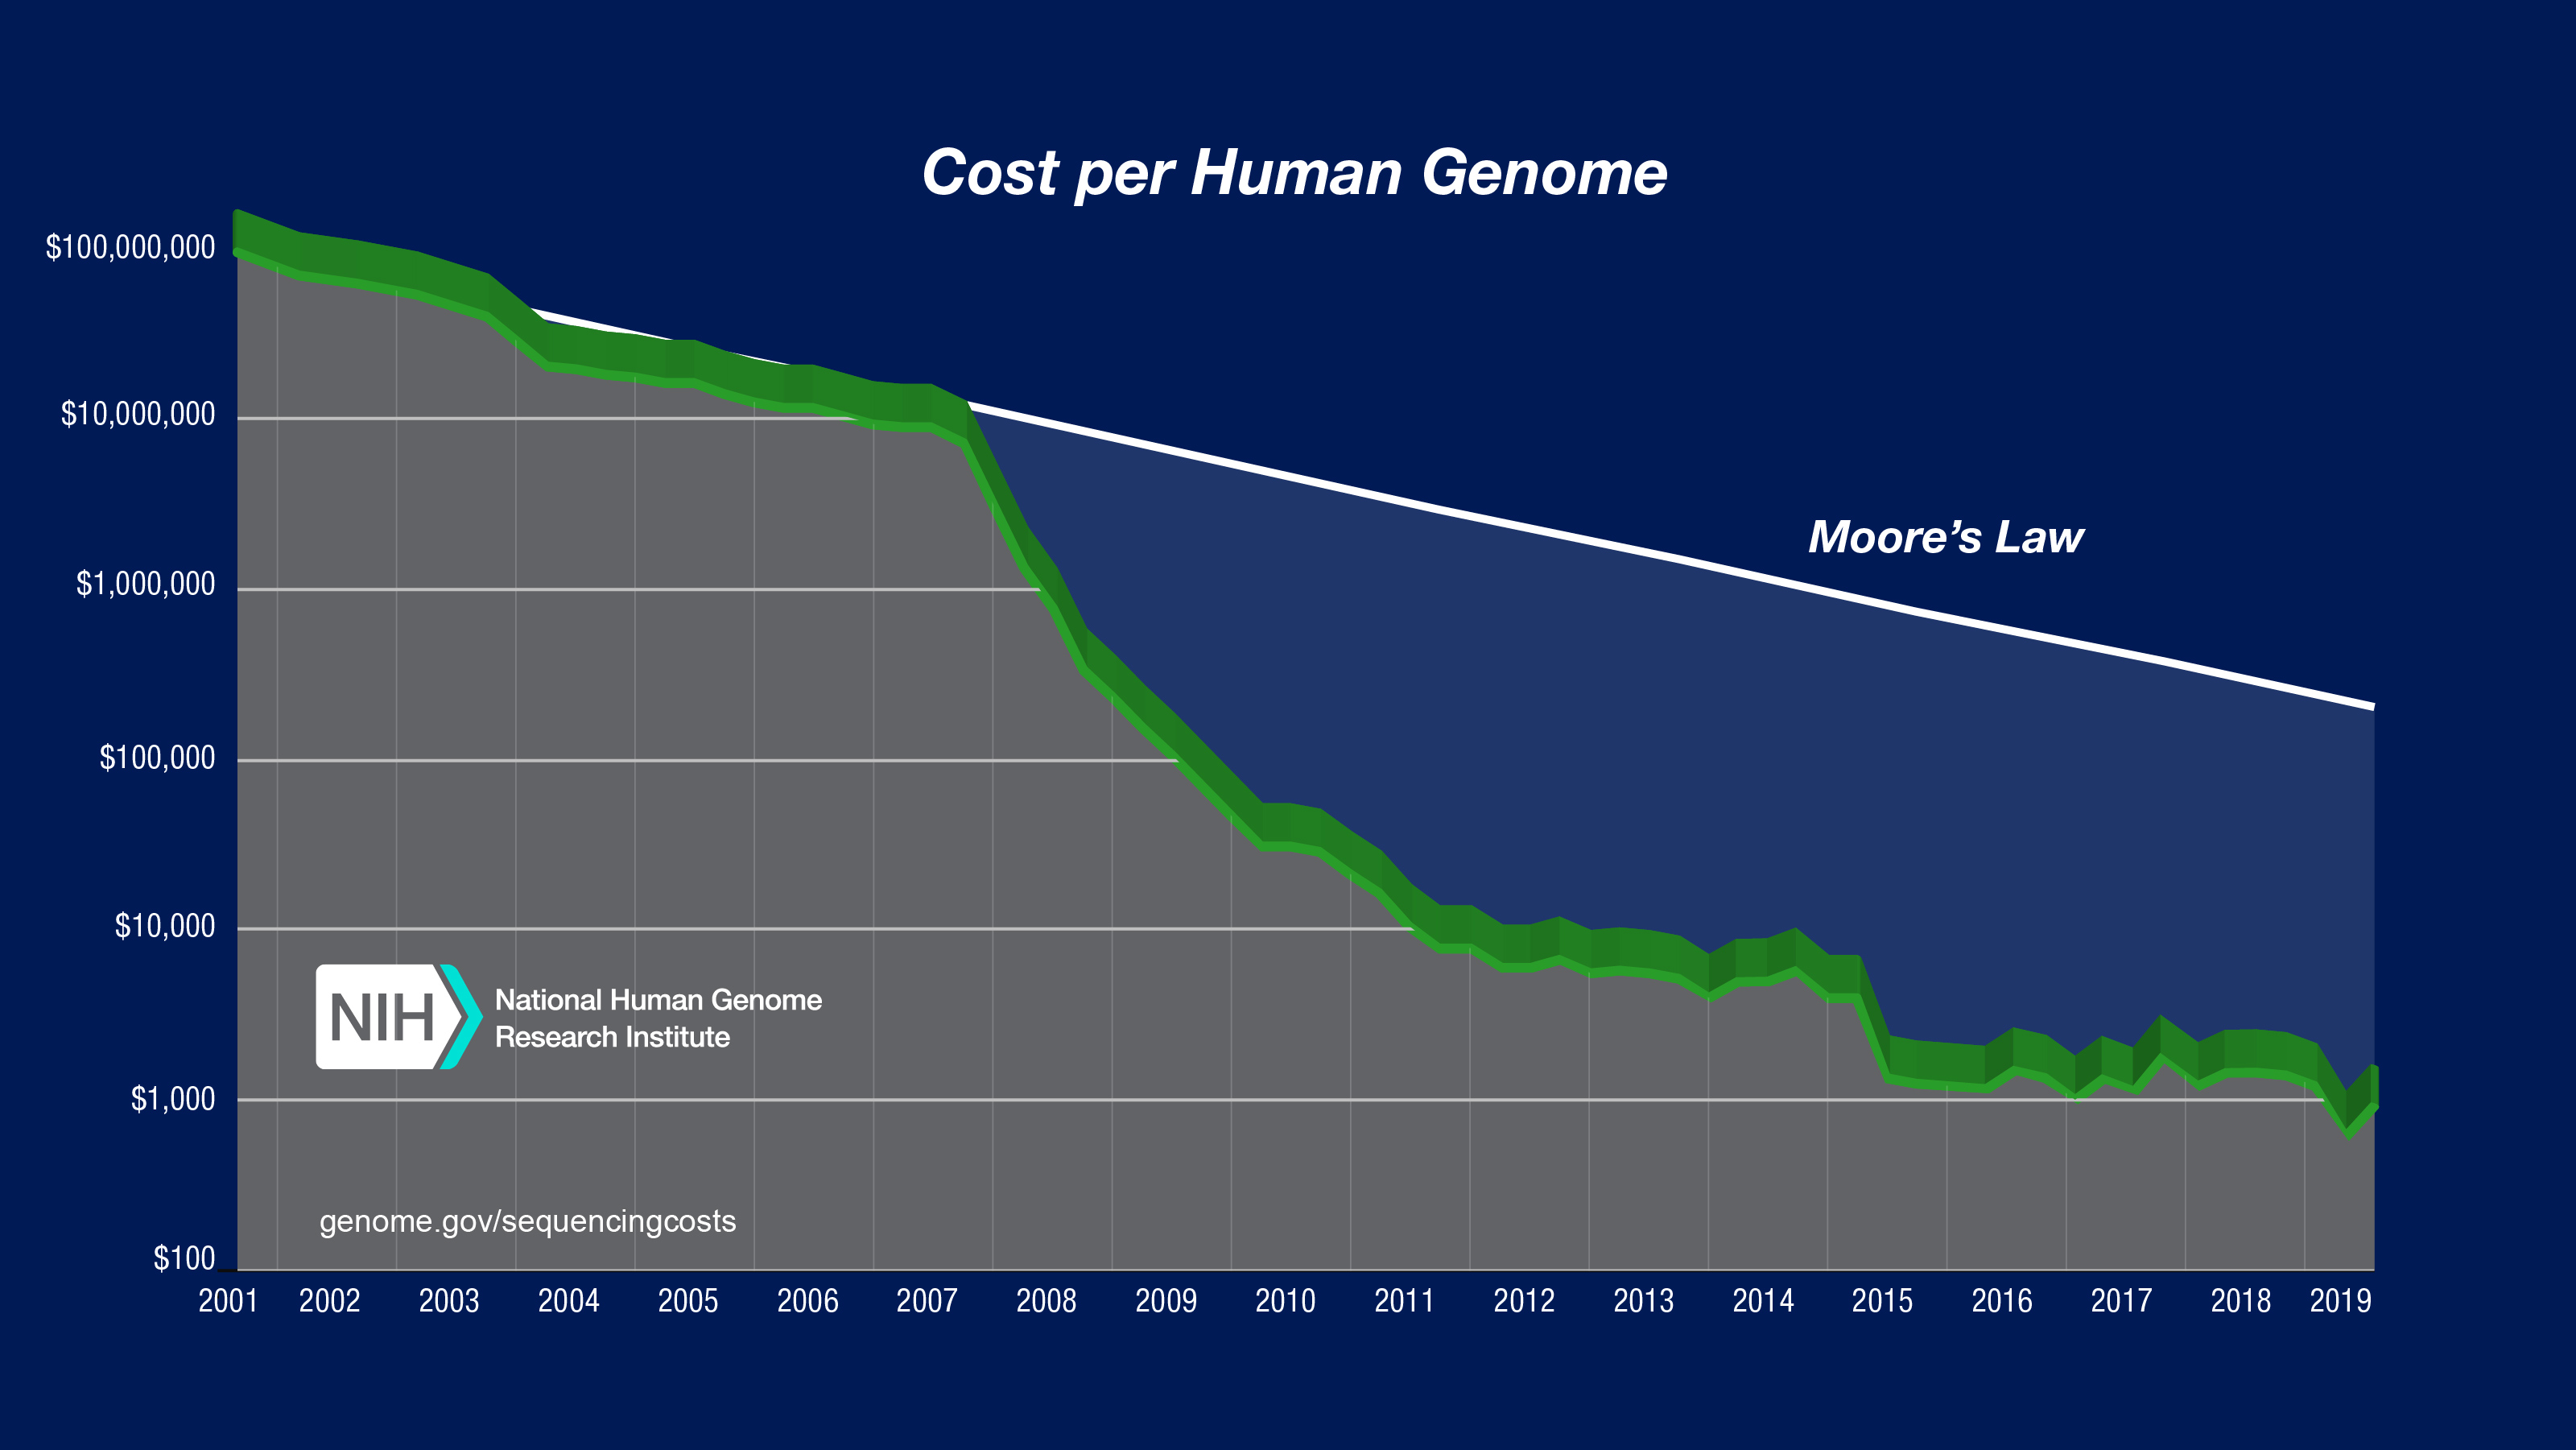
\includegraphics[scale=0.3]{human-gen-cost.jpg}
        
    \end{frame}
    
    \begin{frame}{Sequence data cost over time}
    
    Graph of a megabase sequence cost over time \cite{genomics-cost}
    \begin{itemize}
        \item Megabase means one million bases
    \end{itemize}
    % show how data storage vs production of data
    % get this from hangouts
    \centering
    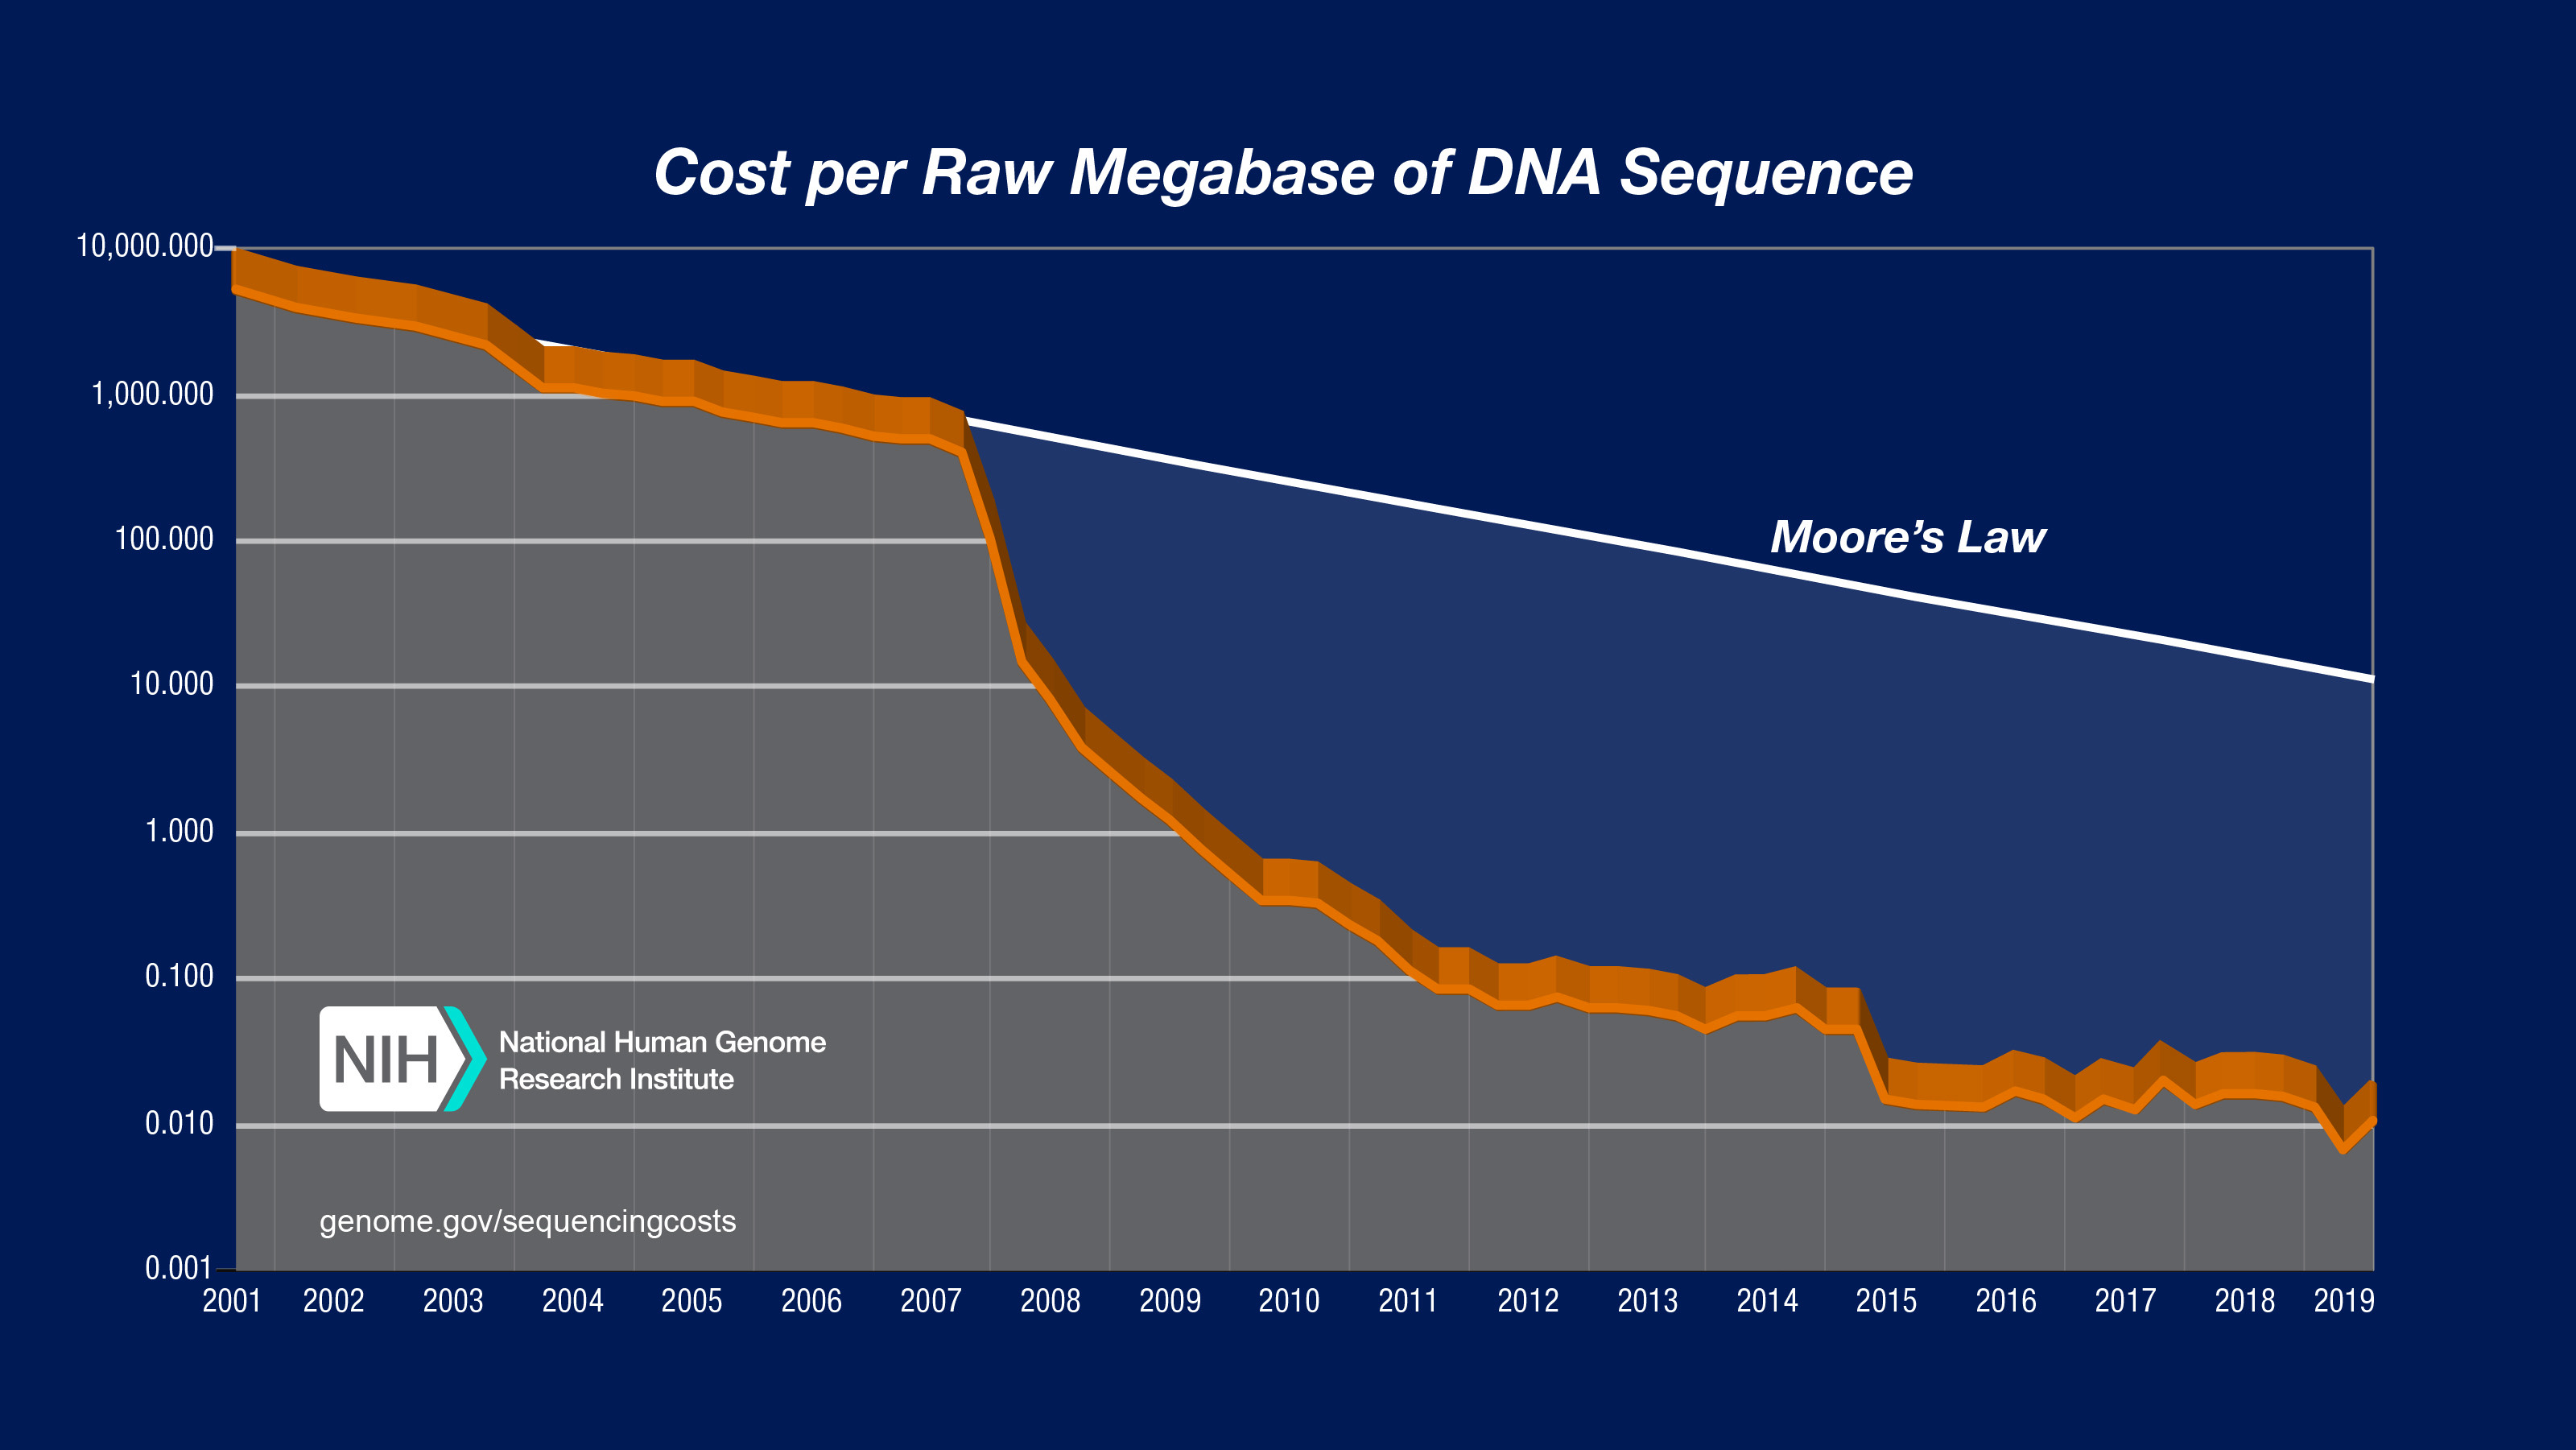
\includegraphics[scale=0.1]{seq-cost.jpeg}
        
    \end{frame}
    
    
    \begin{frame}{NGS vs Hard Disk Storage}
            Computational sense, there is a need to store, upload, and retrieve sequence files that are growing larger. 
            \begin{itemize}
            \item Slope of orange line (NGS) is larger than slope of yellow line (pre-NGS)
            \item Hard disk storage (blue) graph is greater than yellow (pre-NGS) but is now less than orange (NGS)
            \end{itemize}
            \centering
                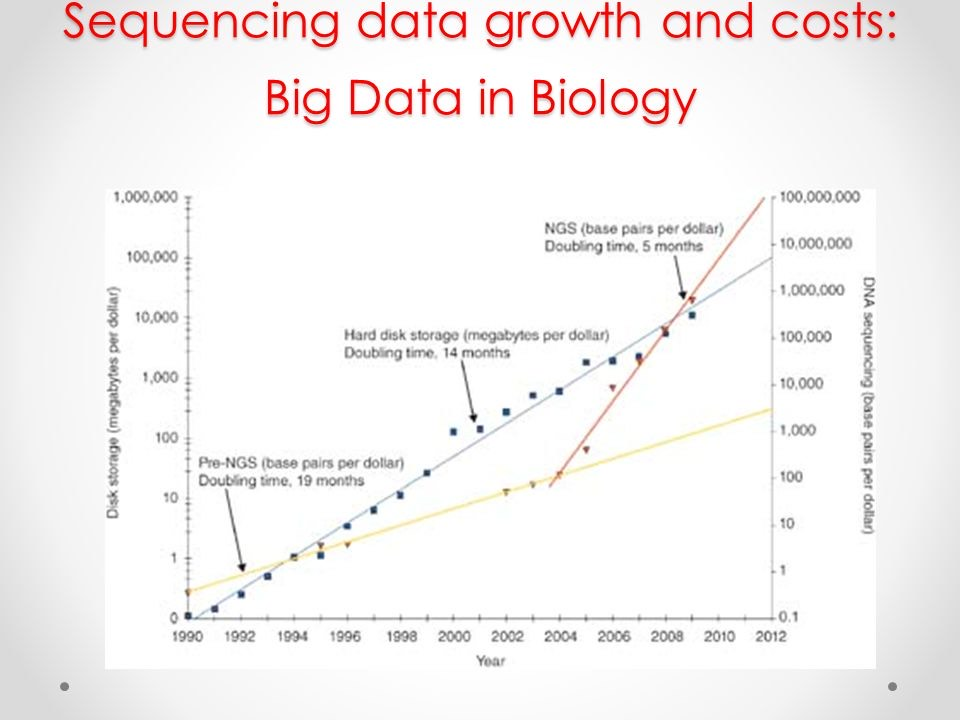
\includegraphics[scale=0.2]{seq-data.jpeg}

    \end{frame}
    

    \subsection{Data Storage}
    \begin{frame}{Data Storage}
        A \textbf{database} (\textbf{DBMS}, Database Management System) is defined by 
        \begin{block} {\textbf{Definition}}

        DBMS contains information about a particular enterprise
        \begin{itemize}
            \item Collection of interrelated data
            \item Set of programs to access the data 
            \item An environment that is both convenient and efficient to use
        \end{itemize}
        \cite{Silberschatz2010}
        \end{block}
    \end{frame}
    
    \subsection{Database Principles}
    \begin{frame}{Database Principles}
        \begin{itemize}
            \item \textbf{Principles} to remember when creating a database (CAP). Idea is that only 2 of the three can be focused on. \cite[Ch.~19]{Silberschatz2010}
            \begin{itemize}
                \item \textbf{Consistency}
                \begin{itemize}
                    \item Update one part, will all other (replicated) parts be updated quickly as well
                    \item Data is accurate and copied faithfully
                \end{itemize}
                \item \textbf{Accessibility}
                \begin{itemize}
                    \item How easy it is to access data
                    \item API protocols
                \end{itemize}
                \item  \textbf{Partition Tolerance}
                \begin{itemize}
                    \item If one portion breaks, the other portions are still usable
                    \centering 
                    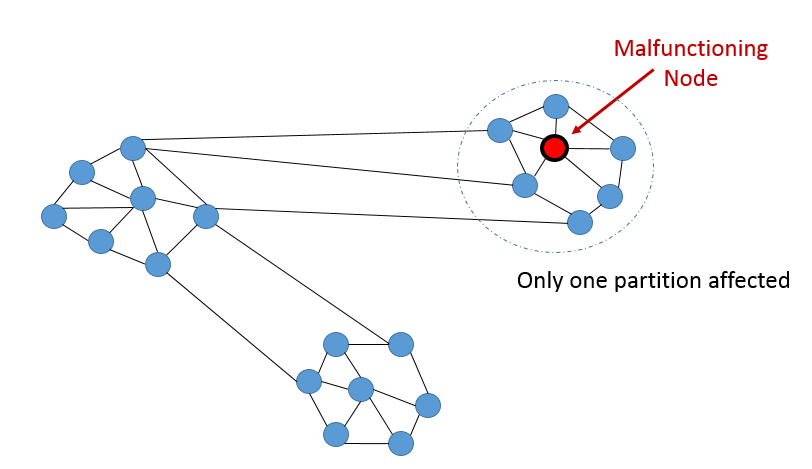
\includegraphics[scale=0.2]{partition_tolerance.png}
                    \end{itemize} 
             \end{itemize}
        \end{itemize}
    \end{frame}
    
    
    %given these efforts, one way to solve it is to have distributed databases, dito pwede pumasok
    
    % dito pwede pumasok yung nireview na technology
    % in presetation di to yung specific section (RRL, Intro)
    % presentation, mas mahalaga yung flow
    % show subsection in a footer, no defined header
    
    \begin{frame}{Normal: NCBI}
        \begin{itemize}
            \item NCBI has a large collection of genomic datasets in its website, which can be searched and downloaded.
        \end{itemize}
    \end{frame}
    \begin{frame}{Normal: NCBI}
        \begin{itemize}
            \item Search page https://www.ncbi.nlm.nih.gov/nucleotide
            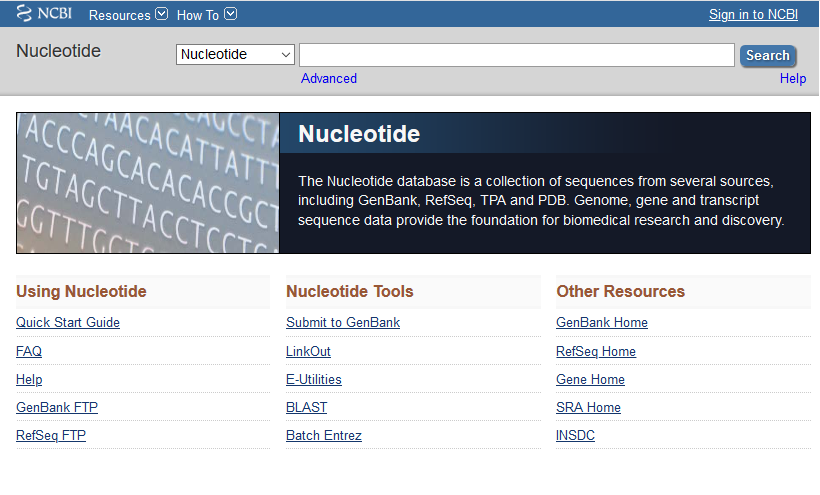
\includegraphics[scale=0.5]{ncbi1.png}
        \end{itemize}
    \end{frame}
    \begin{frame}{Normal: NCBI}
        \begin{itemize}
            \item List of results
            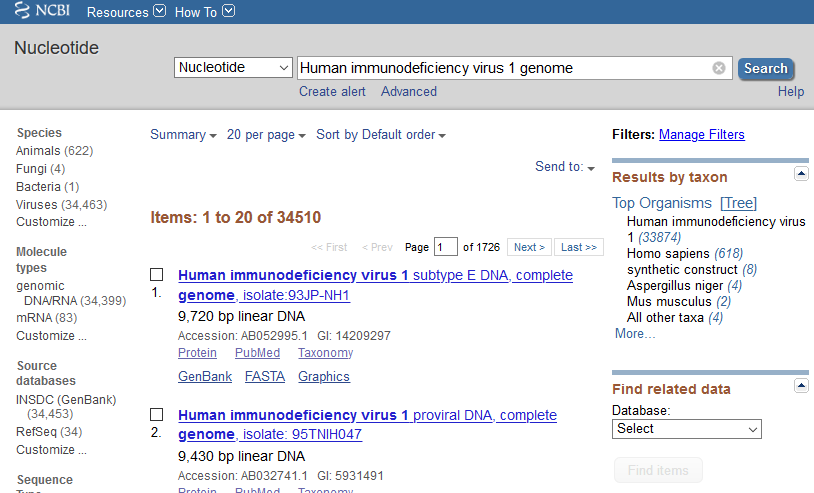
\includegraphics[scale=0.5]{ncbi2.png}
        \end{itemize}
    \end{frame}
    \begin{frame}{Normal: NCBI}
        \begin{itemize}
            \item Download page
            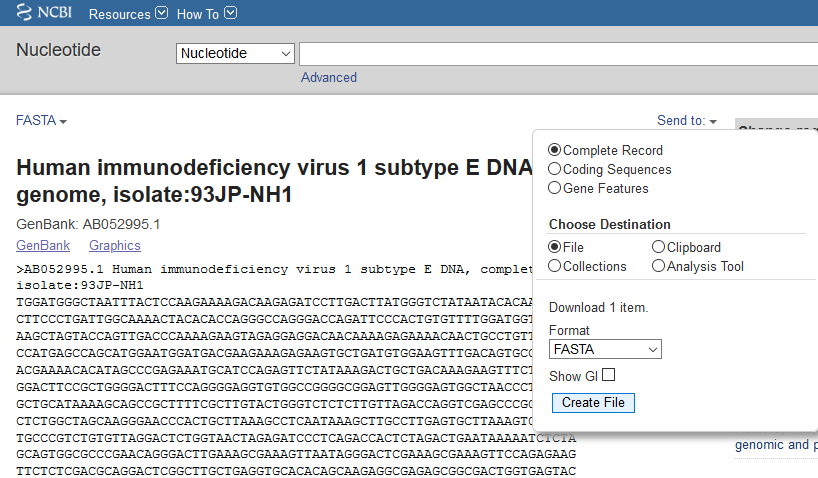
\includegraphics[scale=0.5]{ncbi3.png}
        \end{itemize}
    \end{frame}
    
    
    % cinomment out ko kasi meron naman explanation sa taas
    %\subsection{P2P Database}
    %\begin{frame}{P2P Databases}
    %    something explaining briefly p2p databases
    %\end{frame}
    
        \subsection{BioTorrents}
    \begin{frame}{P2P: BioTorrents}
        \begin{itemize}
            \item Scientific data continues to grow, and so does the demand for easier accessibility
            \item Centralized servers using HTTP or FTP cannot keep up with concurrent requests
            \item Peer-to-peer protocols does not scale well for large files
            \item BitTorrent handles both these problems
        \end{itemize}
    \end{frame}
    
    \begin{frame}{P2P: BioTorrents}
        \begin{itemize}
        \item System for legally sharing scientific data that works on top of the BitTorrent protocol. It is much like a public tracker.
        \item The main website hosts .torrent and metadata files
        \item Info about each dataset includes categories, license, filenames, etc. that helps users in searching for relevant datasets
        \item Torrent file has list of trackers, servers that "know" which peers are serving which files.
        \item Torrent client downloads from multiple peers simultaneously.
        \item To upload a torrent, the client makes a .torrent file using the torrenting software, then uploads it to the main website along with metadata. The client must have their computer continuously turned on to keep the file available as a peer. \cite{biotorrents}
        \end{itemize}
    \end{frame}
    
    \begin{frame}{P2P: BioTorrents}
        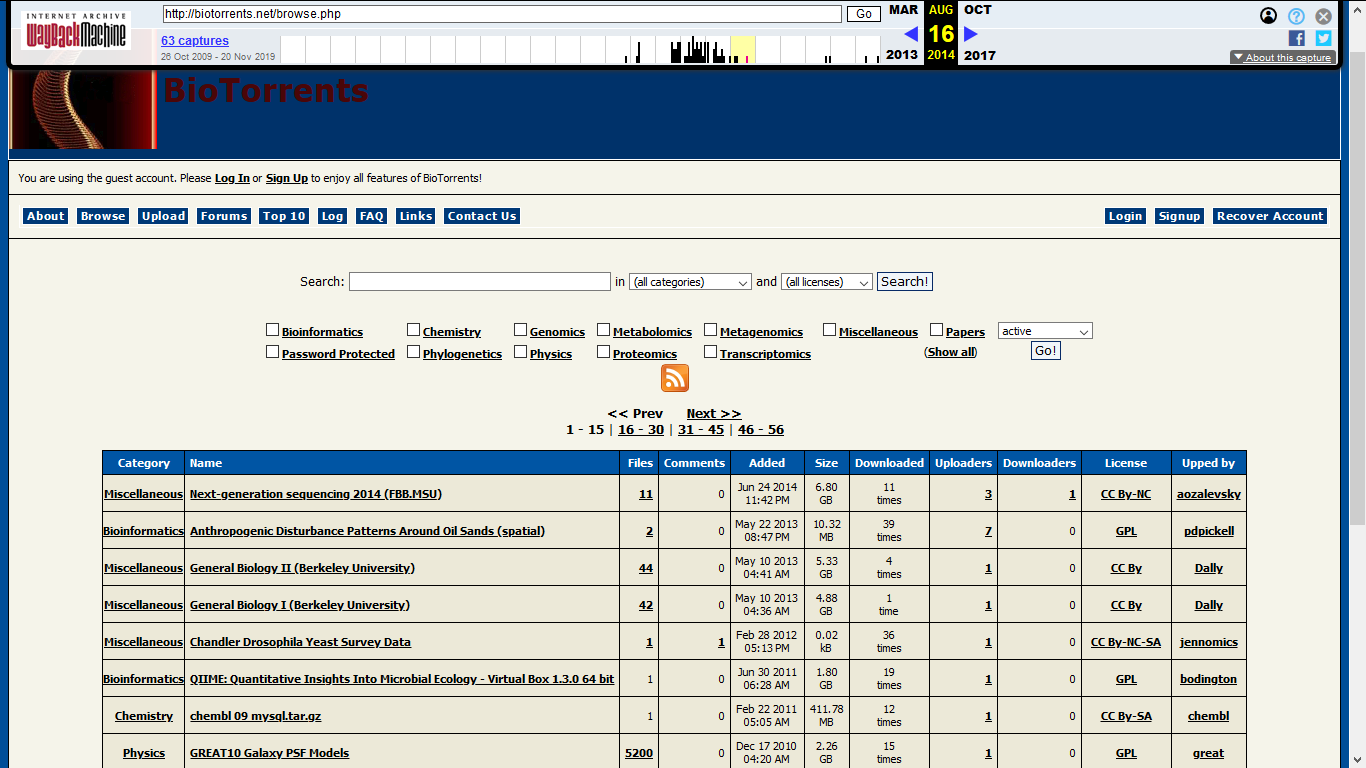
\includegraphics[scale=0.33]{biotorrents-page.png}
    \end{frame}
    
    \begin{frame}{P2P: BioTorrents}
        \begin{itemize}
            \item As with all public trackers, BioTorrents requires "good souls" that will keep many torrents available as often as possible.
            \item The datasets must be moderated to prevent abuse.
            \item The BioTorrents website is no longer up.
        \end{itemize}
    \end{frame}
 
    
    \subsection{PeerDB}
    \begin{frame}{P2P: PeerDB}
    % try adding screenshots
        \begin{itemize}
            \item Proposed P2P system for sharing general data
            \item Each node is equipped with a database
            \item Queries are passed around neighbors, with a maximum number of hops
            \item Caches information about other peers to speed up queries
            \item Large number of nodes \& relatively small number of lookup servers
            \cite{peerdb}
        \end{itemize}
    \end{frame}
    
    \subsection{Distributed Database}
    \begin{frame}{Distributed Databases}
        \begin{itemize}
            \item \textbf{Distributed Database}
            \begin{itemize}
                \item A distributed database system consists of loosely coupled sites that share no physical component             
                \item Database systems that run on each site are independent of each other
                \item Transactions may access data at one or more sites
                \cite[Ch.~19]{Silberschatz2010}
                \item Beneficial for large data with a certain speed requirement
            \end{itemize}
        \end{itemize}
    \end{frame}

        
    \subsection{SeqTorr}
    \begin{frame}{Distributed: SeqTorr}
    \textbf{SeqTorr} \cite{seqtorr}
    \begin{itemize}
        \item Standard genomics workflow consists of uploading and downloading data on an international database like NCBI.
        \item Having a distributed scalable local infrastructure to store genomic data instead of relying on NCBI would be beneficial since
        \begin{itemize}
            \item only certain sequences in NCBI are relevant to the institutions (e.g. Asian sequences are needed more than Caucasian ones)
            \item researchers within the country can share data with fast speeds
            \item institutions can share in the hosting of data
        \end{itemize}
    \end{itemize}
    \end{frame}
    \begin{frame}{Distributed: SeqTorr}
    \begin{itemize}
        \item Utilizes distributed database
        \item Master node
        \begin{itemize}
            \item containing metadata of all the sequences
            \item where user authentication is handled
        \end{itemize}
        \item Data node
        \begin{itemize}
            \item contain a portion of all the sequences
            \item needs to replicate a sequence \texttt{r} times before a sequence is considered available
            \item proximity of data nodes can increase download speed
        \end{itemize}
        \item Defined API Implementation
        \begin{itemize}
            \item POST
            \item GET
            \item PUT
            \item DELETE
        \end{itemize}

    \end{itemize}
    \end{frame}
    
    
    \begin{frame}{Distributed: SeqTorr}
    % have a unified way of discussing each database
    % what aspects of the database to discuss each
    % extra features will come after
        Problems: % have one for each database system
        \begin{itemize}
            \item program not currently available
            \begin{itemize}
                \item cannot measure any statistics on this
            \end{itemize}
        \end{itemize}
    \end{frame}
    



    
\begin{frame}{Table}
% Bio-related -> biological
% What's the difference between biological vs general vs FASTA
% What does general mean?
% What does biological mean? -> explain pa to
% May 3 types of data ...
   \begin{table}[]
        \begin{tabular}{|l|l|l|l|l|}
        \hline
        System      & CS/P2P/H & Available? & DL/UL speed & Type of Data \\ \hline
        BioTorrents & P2P           & No         & Depends                    & Biological  \\ \hline
        SeqTorr     & H             & No         & Fast (PH server)           & FASTA        \\ \hline
        PeerDB      & P2P           & No         & Depends                    & General      \\ \hline
        NCBI        & CS            & Yes        & Slow (US server)           & Biological  \\ \hline
        \end{tabular}
    \end{table} 
\end{frame}


%%%%%%%%%%%%%%%%%%%%%%%%%%%%%%% PROBLEM %%%%%%%%%%%%%%%%%%%%%%%%%%%%%%%%%%%%

\section{Problem}
% after discussion of dist. databases
\begin{frame}{Problem}
The different gaps or problems found with other implementations
\textbf{Problems of Classical Databases}
\begin{enumerate}
%PROBLEMS OF CLASSICAL DATABASES (ALL FOUR)
    \item Genome researchers download entire database of genomic data
    \item Genome researchers only need a portion of the database, but end up downloading everything  (gigabytes size)
    \item Client-Server approach can face bottlenecks (server speed) %is resolved by making it more distributed
    \end{enumerate}
% or having a hard time getting a portion of the database
% easier to download parts vs whole, whole vs parts

% not easy to navigate the database? 
% what is the big problem? too big data to download all at once?
% why is it a problem? speed of download? or size?

\textbf{Problems of Distributed Databases}

\begin{enumerate}
%PROBLEM OF DIST. DATABASES
    \item Only one framework on distributed database for genomes
    \item Existing distributed database for genome code has little documentation % concept of APIs and documentation

\end{enumerate}
\end{frame}

%%%%%%%%%%%%%%%%%%%%%%%%%%%%% TITLE %%%%%%%%%%%%%%%%%%%%%%%%%%%%%%%%%%%%%%%%%%%%%%
\begin{frame}
\titlepage % Print the title page as the first slide
\end{frame}


%%%%%%%%%%%%%%%%%%%%%%%%%%%%%%%%%%%%% OBJECTIVES %%%%%%%%%%%%%%%%%%%%%%%%%%%%%%%%%%%%%%%%

\section{Objectives}
% to tackle those problems
% should be written in connection with the problems said:
% problem x : objective x
% para mas clear yung objectives

\begin{frame}{Objectives}
Based on the problems we found earlier, we propose the following objectives
 \begin{itemize}
    \item Create an information system that speeds up the download and upload of genomic data
    \begin{itemize}
        \item To resolve 1 \& 2 of the Problems of Classical Databases. 
    \end{itemize}
\end{itemize}

\begin{itemize}
    \item The system should have the main API’s
    \begin{itemize}
        \item POST genome data
        \item GET genome data (implement hybrid P2P)
        \begin{itemize}
            \item This will aim to resolve number 3 in the Problems of Classical Databases
        \end{itemize}
        \item PUT genome metadata (optional: PUT data)
        \item DELETE genome data
    \end{itemize}
    \item Write documentation for the system
    \begin{itemize}
        \item This will be used to resolve the Problems of Distributed Databases
    \end{itemize}
\end{itemize}
\end{frame}

\section{Scope}
\begin{frame}{Scope}
The current scope and coverage of the project is only
\begin{itemize}
    \item Security and Authentication is not part of the scope
    \item Use only FASTA file format 
    \begin{itemize}
        \item DNA nucleotides only
    \end{itemize}
    \item Only a proof of concept, UI will be purely for functional purposes (very basic design)
\end{itemize}
\end{frame}

%%%%%%%%%%%%%%%%%%%%%%%%%%%%%%%%%%%%%% THEORETICAL FRAMEWORK %%%%%%%%%%%%%%%%%%%%%%%%%%%%%%%%%%

\section{Theoretical Framework}
% dito idiscuss yung tech
% ito ipopropose namin 
% lahat ng network layers, client-servers


        \begin{frame}{Network Layers}
        % not part of intro na 
        % pwede sa methods / theoretical framework na iintroduce
        % medyo off sa flow
         \textbf{Networks Layers} how computers pass data to each other
        \begin{itemize}
            \item \begin{itemize}
            \item Level 1: Medium used to send signals (physical, electrical signals of 0 and 1), through wire or by air
            \item Level 2: Introduction of packets: Wifi, Ethernet, connecting together different . Goal of sending a group of signals.
            \item Level 3: Introduction of networks: IP Address to uniquely identify entities. 
            \item Level 4: Management of error free data transmission: Sending a group of messages via TCP, UDP, FTP
            \item \textbf{Level 5}: Abstraction of Level 4: Function calls programmers will use to do level 4 processes.
            \end{itemize}
        \end{itemize}
    \end{frame}
    
    \subsection{Application Architecture}
    % part ng theoretical framework
    % pwedeng walang slide of c/s
    % pwedeng ibanggit nalang ang client-server architecture

    % methods: ito framework
    % implemens client-server...
    \begin{frame}{Application Architecture}
        \begin{itemize}
            \item The \textbf{application architecture} is how a networked app is structured across the various end systems (i.e. computers, servers, etc.) \cite{kurose}
            \item Falls into either client-server, peer-to-peer, or hybrid architecture
        \end{itemize}
    \end{frame}
       
       
        \subsubsection{Client-Server}
        \begin{frame}{Client-Server}
            \begin{itemize}
                \item A \textbf{client-server} architecture relies on a Web server that is always available and has a fixed IP address\\
                \item A single server connects to many clients
            \end{itemize}
            \centering
            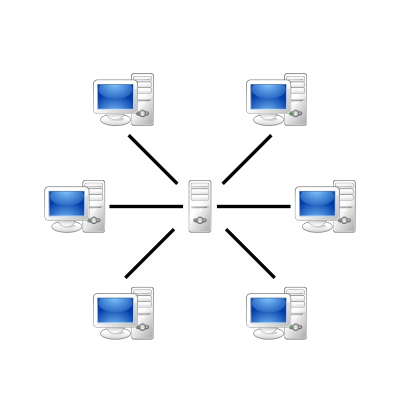
\includegraphics[scale=0.5]{Server-based-network.png}
        \end{frame}
       
       
        \subsubsection{Peer-to-Peer \& Hybrid}
        \begin{frame}{Peer-to-Peer \& Hybrid}
            \begin{itemize}
                \item A \textbf{peer-to-peer (P2P)} architecture has minimal to no reliance on always-on, dedicated servers
                \item Peers are desktops/laptops that communicate to each other without passing through a dedicated server
                \item A \textbf{hybrid} architecture combines elements of P2P and client-server architectures, attempting to utilize advantages of both
            \end{itemize}
            \centering
            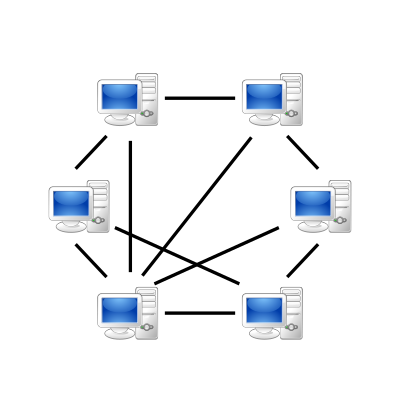
\includegraphics[scale=0.5]{P2P-network.png}
        \end{frame}
        
        \begin{frame}{Bittorent terminology}
            % ADD SCREENSHOT
            Peers \\ \\ 
             \centering
            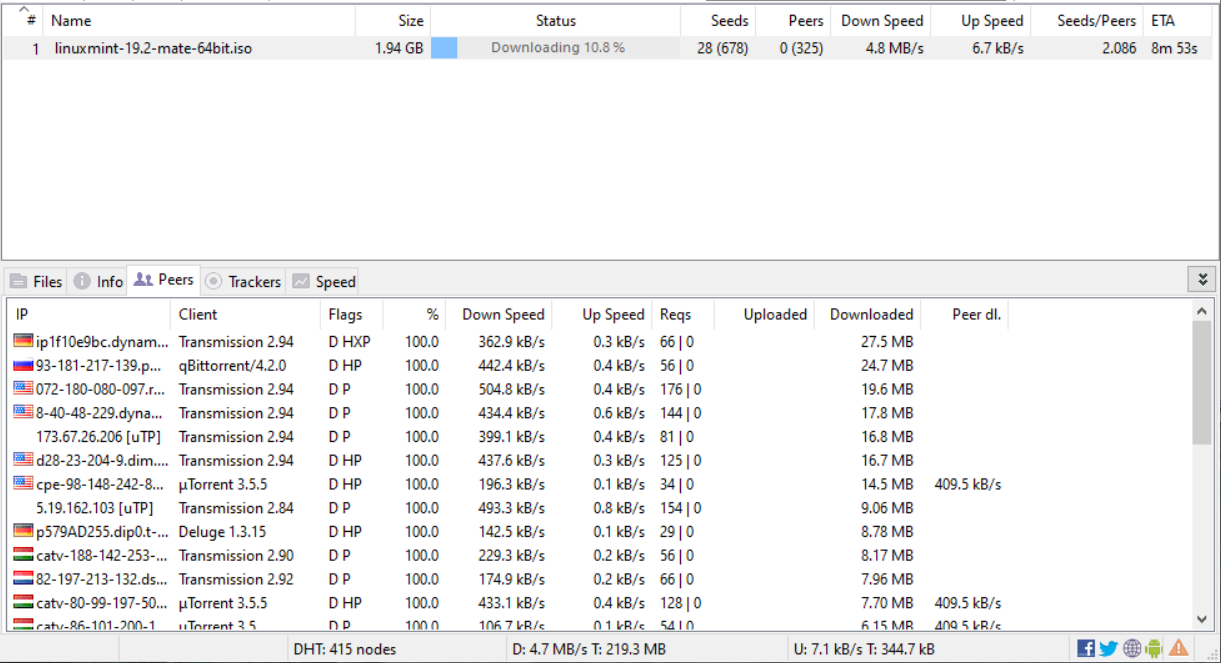
\includegraphics[scale=0.5]{bit-2.PNG}
        \end{frame}
        
        \begin{frame}{Bittorent terminology}
            % ADD SCREENSHOT
            Trackers \\ \\
             \centering
            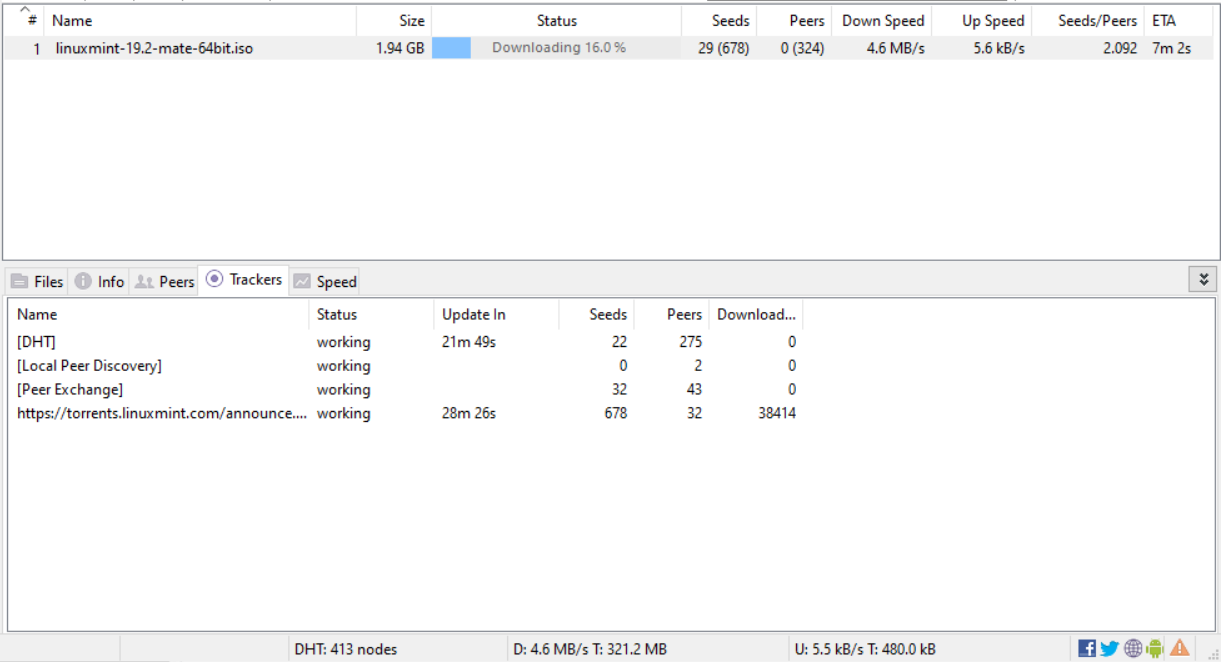
\includegraphics[scale=0.5]{bit-3.PNG}
        \end{frame}
        
        \begin{frame}{BitTorrent terminology}
            % visually show each term din
            % screenshot of torrent
            \begin{itemize} % siguro breeze through what these mean 
                \item \textbf{Peers} are users that connect to the BitTorrent network.
                \item \textbf{Torrent files} contain metadata about files \& folders, trackers, and hash values.
                \item \textbf{Trackers} are servers that keep track of peers and availability of files
                \item \textbf{Seeds} are peers which have downloaded the entire file and are making it available
            \end{itemize}
        \end{frame}




\begin{frame}{Theoretical Framework: System Description}
    \begin{itemize}
        \item A \textbf{master node} stores metadata of all sequences, may or may not contain sequence files
        \item \textbf{Data nodes} stores sequence files \& metadata of all sequence files in its filesystem
        \item Both master node \& data nodes have user interface that allow users to upload, search, and download sequence files
    \end{itemize}
\end{frame}

% DRAW.IO FILE: https://drive.google.com/file/d/1Nbp0Kmgcr2BZ13LBT3SGLMBoA6JA_Eth/view
\begin{frame}{Theoretical Framework: Schematics}
\textbf{App network diagram} \\ \medskip
\centering
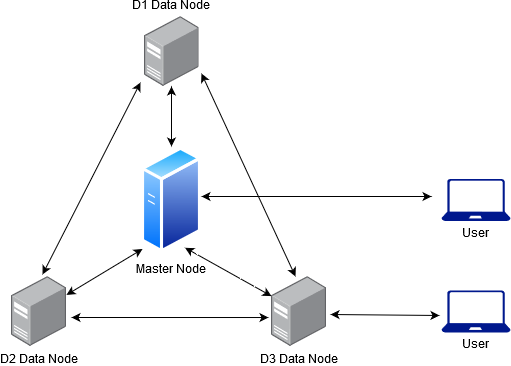
\includegraphics[scale=0.5]{thesis1.png}
\end{frame}

\begin{frame}{Theoretical Framework: Schematics}
\textbf{POST: Uploading a sequence to the master node} \\ \medskip
\centering
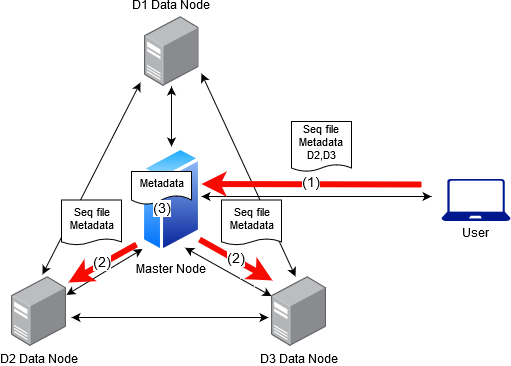
\includegraphics[scale=0.5]{thesis3.png}
\end{frame}

\begin{frame}{Theoretical Framework: Schematics}
\textbf{POST: Uploading a sequence to a data node} \\ \medskip
\centering
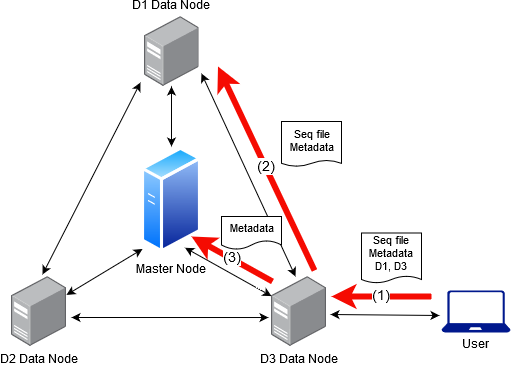
\includegraphics[scale=0.5]{thesis2.png}
\end{frame}

\begin{frame}{Theoretical Framework: Schematics}
\textbf{GET: Downloading a sequence} \\ \medskip
\centering
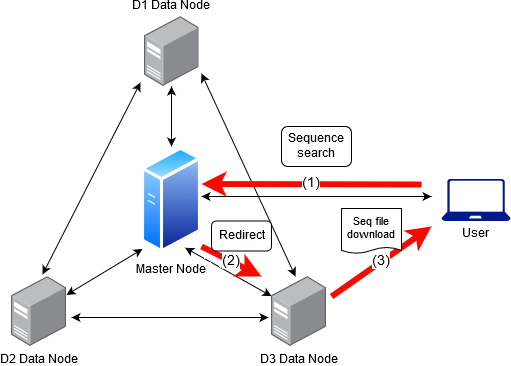
\includegraphics[scale=0.5]{thesis4.png}
\end{frame}

\subsection{Data Model}
\begin{frame}{Data Model}
%% GET THIS FROM SEQTORR

% So far the data stored will be 1 table
% Sequence, Author, Institution, Species, Chromosome, Chromosome Position, Date -> CHECK SEQTORR
% Part of Theo Framework
This data model is lifted from SeqTorr \cite{seqtorr}


\small
\begin{center}
    

\begin{tabular}{c|c}
\hline
    key & description \\
\hline
\hline
    seq\textunderscore id & unique ID assigned to all sequences \\
    organism & organism where the sequence was extracted from \\
    quality & the rating of the data based on the number of downloads or another criteria \\
    uploader & user that uploaded the data \\
    institute & institute where the uploader or sequence was taken from \\
    upload\textunderscore date & date the data was uploaded to the database \\
    last\textunderscore modified & the date the metadata or data was edited \\
    data\textunderscore nodes & list of data nodes that this data contains
\end{tabular}
\end{center} 


\end{frame}

\subsection{Data Permissions}
\begin{frame}{Data Permissions}
% Uploading can be done by anyone (easily)
% But only master (we can call it moderator) can screen and verify
% Anyone can download -> has to be a hash sum to verify integrity of contents
% Users - Moderator, Users / Peers
% Part of Theo Framework
% EXPLAIN ^^ NALANG

% Data Integrity - Makes sure data downloaded is always consistent -> use hashing algorithms, save the hash in the master file, checksum / hash

% merong private 
% -> kahit sa UI lang siya magauthenticate
% -> sa table lang nakasabi sino may access (just an added column)
% merong public
\begin{center}
\begin{tabular}{c|c}
\hline
    user & description \\
\hline
\hline
   Moderator & Has ability to upload, download, store data, verify \\
    Peer & Has ability to upload, download, store data \\
    Guest & Has ability to upload, download \\

\end{tabular}
\end{center}

\end{frame}

% where does data pass through (schematic)

%%%%%%%%%%%%%%%%%%%%%%%%%%%%%%%% PROPOSED METHODOLOGY %%%%%%%%%%%%%%%%%%%%%%%%%%%%%%%%%%%%%%
\section{Proposed Methodology}
\begin{frame}{Proposed Methodology}
\begin{enumerate}

% have 3 subsections, each of those tasks, turn into sentences
% try to identify tools per task (or possible tools)
    \item Creating the system
    \begin{enumerate}
        \item Code data node
        \item Deploy \& test functionality of data node/s
        \item Code master node
        \item Deploy \& test functionality of master node/s
        \item Test interoperability of nodes
    \end{enumerate}
    \item Benchmarking
    \begin{enumerate}
        \item Create test for testing original speed
        \item Test original download speeds
        \item Create test for testing new speed
        \item Test new speeds
    \end{enumerate}
        \item Documentation
    \begin{enumerate}
        \item PDF \& Github Style
        \item How to use (all users)
        \item How to set up
        \item How to maintain \& add features
        \item How to test?
    \end{enumerate}
\end{enumerate}
\end{frame}

%Proposed tech background -> paper
% Visualize Gantt Chart
% Cluster together the parts
% Gantt chart nalang
% As early as possible
% Try transfer between nodes, com sci -> PGC


%GAMEPLAN
%pagnaset up kaagad
%check speedup, kahit sobrang pangit basta may speedup
%pag may speedup graduate na

%GAMEPLAN
% 1) Working System
% 2) May Speedup
% 3) Tama Data na kinocopy 100% accuracy
% 4) Tama Distribution, ay feature to find fastest route, way to find fastest download piece
% 5) Usability & Documentation
% 6) Authenticaion
% 7) UI



% FIRST WEEK
% choose dataset from ncbi
% time the dataset download
% set this as initial time to beat
% compare between normal file transfer

%%%%%%%%%%%%%%%%%%%%%%%%%%%%%%% TIMELINE %%%%%%%%%%%%%%%%%%%%%%%%%%%%%%%%%%%%%%%%%%%%%%%%%%%%%

\subsection{Proposed Methodology Timeline}
\begin{frame}{Proposed Methodology: Timeline 1}
    \begin{itemize}
        \item Mid January: Start
        \item Mid April: End
    \end{itemize}
    \begin{enumerate}
        \item End January Deliverable: 
        \begin{itemize}
        % start having API calls na
            \item Wireframe Mockup
            \item Pseudocode / Flowchart of Entire System (to be reviewed by the adviser)
            \item Finalized feature list
            \item Documentation Version 1 (Cid)
        \end{itemize}
        \item End of February Deliverable:
            \begin{itemize}
                \item Benchmarking specifications finalization \& Set up
                \item Start of bench marking of existing tech
                \item Start Coding
                \item Documentation Version 2 (Cid)
            \end{itemize}
    \end{enumerate}            
            \end{frame}


    \begin{frame}{Proposed Methodology: Timeline 2}
        \begin{enumerate}  
        \item Mid March Deliverable:
            \begin{itemize}
                \item Finish Coding version 1 of system
                \item Implement basic UI
                \item Finish bench marking existing 
                \item Start Alpha Testing (us and other undergrad thesis students)
                \item Documentation Version 3 (Cid)
            \end{itemize}
        \item End of March Deliverable:
            \begin{itemize}
                \item Revise version 1 to version 2 of system based on Alpha Test
                \item Revise basic UI
                \item Testing of system for feature 
                \item Start Beta Testing (public, DCS \& PGC community)
                \item Documentation Version 4 (Cid)
            \end{itemize}
        \item Mid April Deliverable
            \begin{itemize}
                \item Revise version 2 to version 3 of system based on Beta test
                \item Documentation Version 5 (Cid)
            \end{itemize}
    \end{enumerate}
\end{frame}


    \begin{frame}{Proposed Methodology: Gantt Chart}
        \centering
        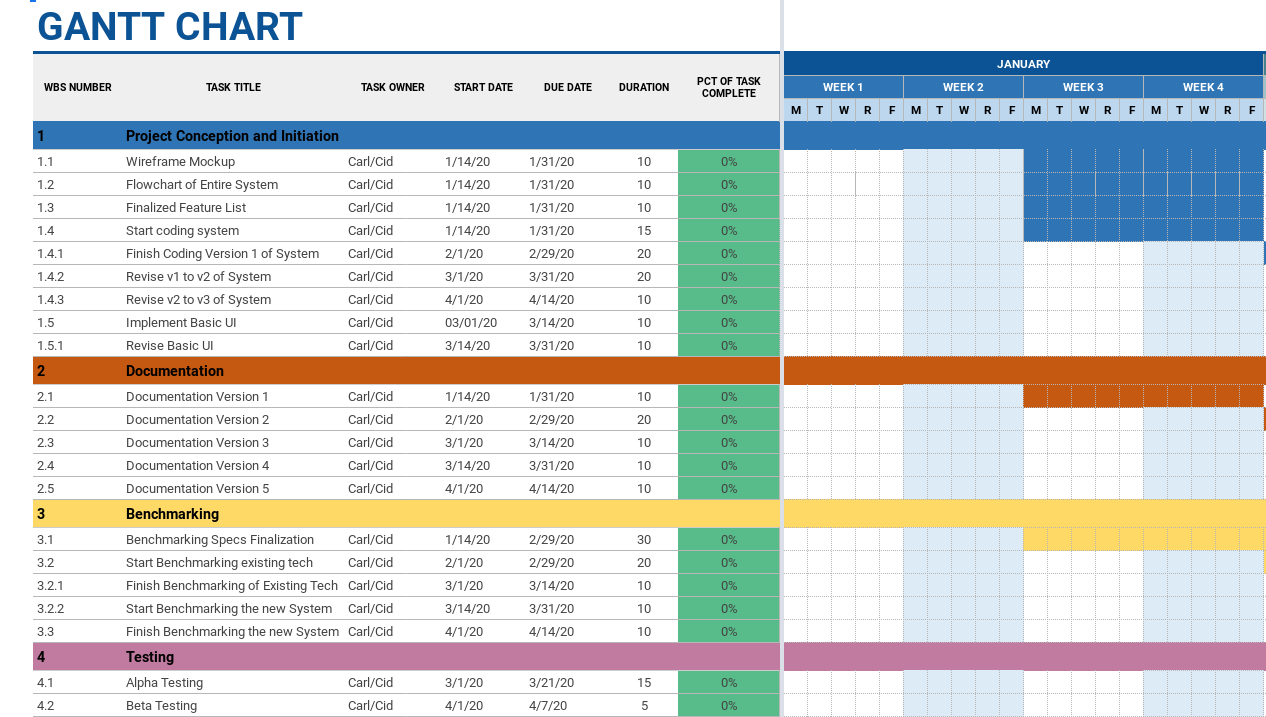
\includegraphics[scale=1]{jan.png}
    \end{frame}
    
    \begin{frame}{Proposed Methodology: Gantt Chart}
        \centering
        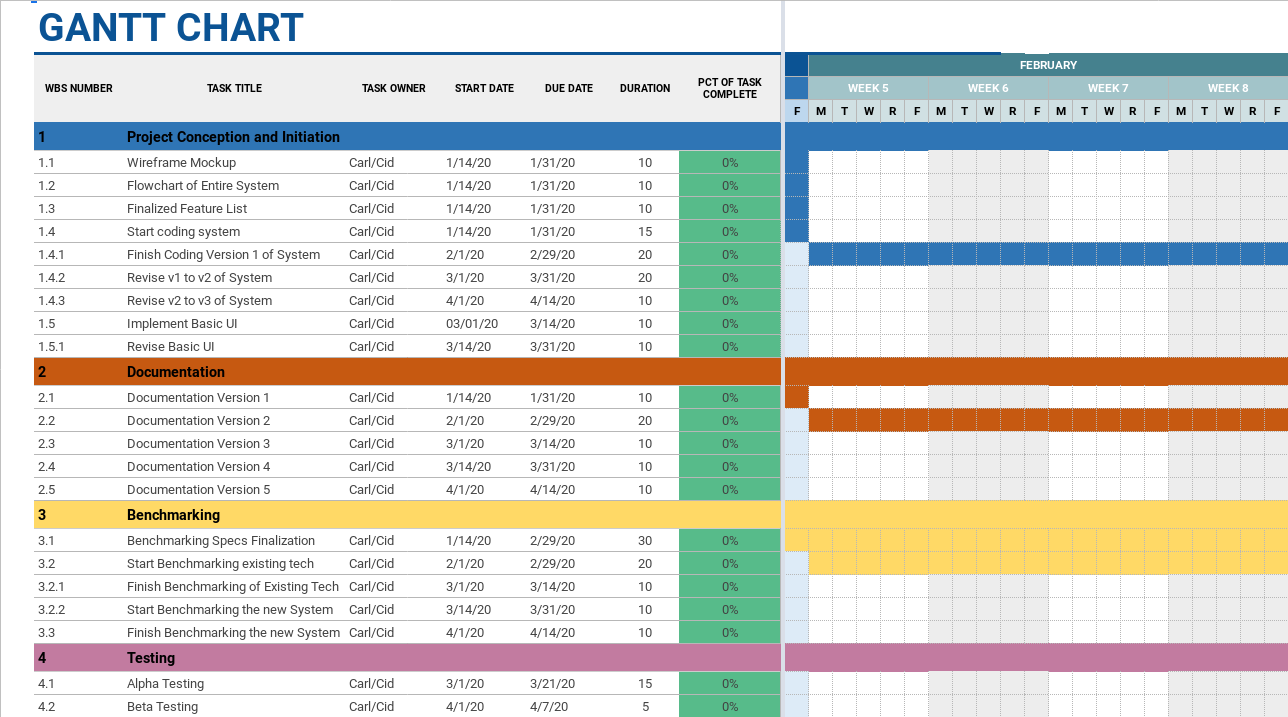
\includegraphics[scale=1]{feb.png}
    \end{frame}
    
    \begin{frame}{Proposed Methodology: Gantt Chart}
        \centering
        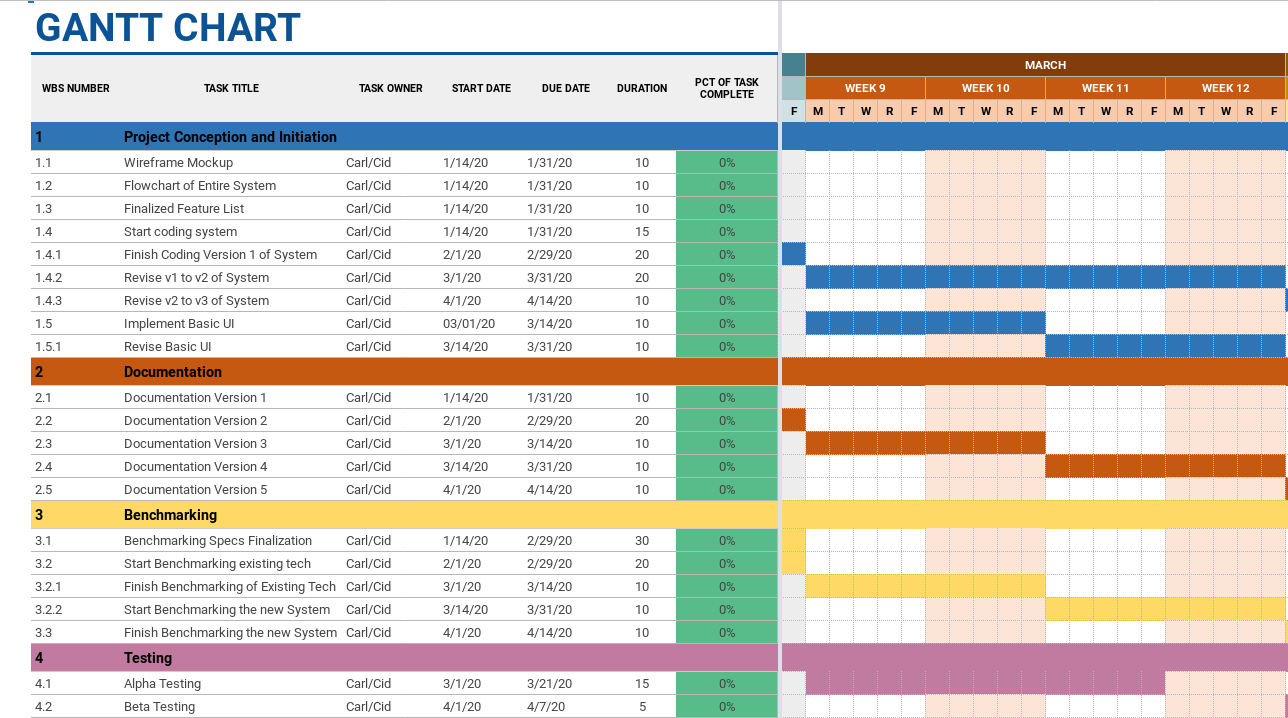
\includegraphics[scale=1]{mar.png}
    \end{frame}
    
    \begin{frame}{Proposed Methodology: Gantt Chart}
        \centering
        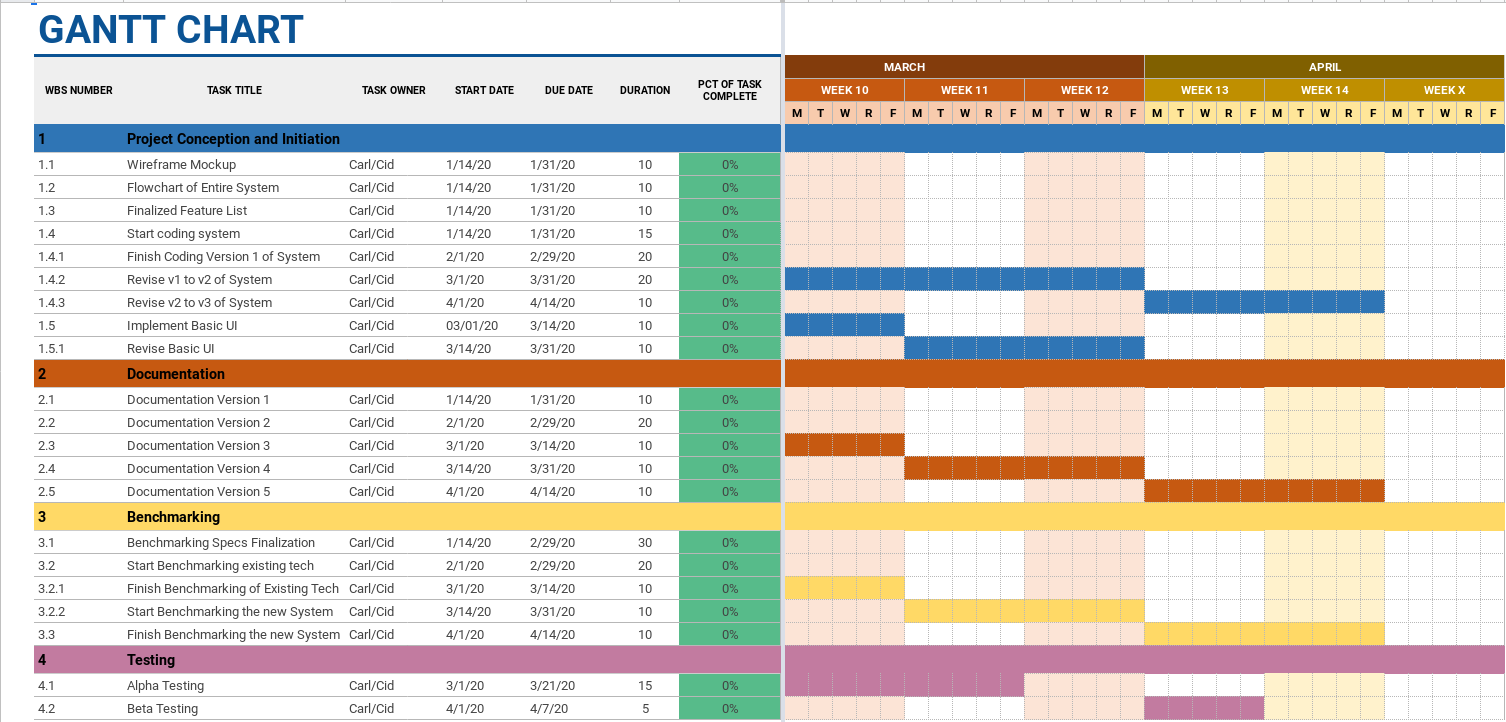
\includegraphics[scale=1]{april.png}
    \end{frame}



\begin{frame}
\Huge{\centerline{The End}}
\small{\centerline{Thank you for coming}}
\end{frame}

\section{Bibliography}

\begin{frame}[allowframebreaks]
\printbibliography[heading=none]
\end{frame}


\end{document}

